\documentclass{article}
\usepackage{amsmath}
\usepackage{graphicx}

\title{Flux Through One Dimensional Slab of Multiplying Media}
\author{J. Jewell \and T. Looby \and A. Salakovich \and J. Starks}
\date{October 31, 2017}

\begin{document}
	\maketitle
	
	\section{Introduction and Background}
			The scope of the assigned project was to prepare a code to numerically determine the flux through a one dimensional slab of a multiplying medium. The critical width was calculated so that k was made to equal 1. The iteratively calculated critical width was comparable to an analytically calculated critical width. 
	\section{Methodology}
		\subsection{Analytical Solution}
			The critical width of a half slab was determined analytically using the buckling terms. For the system to be critical, the material buckling must equal the geometric buckling. 
			
			The material buckling for a system is independent of the geometry and is expressed as follows
			\begin{equation}
			B_{m}^{2}=\frac{\nu \Sigma_{f}-\Sigma_{a}}{D}
			\end{equation}
			
			The geometric buckling, which is independent of the material, for a Cartesian slab is defined as follows where 'a' is the slab width.
			
			\begin{equation}
			B_{g}^{2}=(\frac{\pi}{a})^{2}
			\end{equation}
			
			Setting the two buckling equations equal and solving for the width 'a' yields the critical width of the slab. 
			
			\begin{equation}
			a=\pi \sqrt{\frac{D}{\nu \Sigma_{f}-\Sigma_{a}}}
			\end{equation}
		
			To solve for a critical width for a system of different geometry, only the geometric buckling term must be changed as the material buckling is independent of system geometry. 
		\subsection{Numerical Solution}
			The numerical solution was found to generally agree with analytical results.  Several methods were attempted to maximize convergence and minimize processing time.  Two separate iterations were needed to simultaneously find eigenvalues and critical width .  The objective of the inner iteration was to converge to an eigenvalue, k.  The tolerance for this convergence was varied between 1% and 0.01%.  Once a value of k was determined to be convergent, the outer iteration commenced, with the objective of manipulating reactor width as a means of obtaining a critical system.  Reactivity as a function of width was employed, with the goal of finding a reactivity of 0.  To achieve this width "searching" various methods were attempted.  
			First, a simple linear zero search method was utilized, in which an algorithm incremented or decremented width in predetermined step sizes.  If the reactivity approached zero with each successive iteration, then the step remained unchanged.  If the reactivity grew in either direction, then the polarity of the increment was reversed and the step size halved.  This approach was extremely reliable for finding the critical width, but at the cost of extremely slow convergence times.  As a means of decreasing convergence time, the Newton Raphson was implemented.  In this algorithm, the derivative of the reactivity is calculated for each iteration, and a zero is discovered via linear interpolation.  This method enabled faster convergence, yet has limitations.  If the initial guess for reactor size is not proximal to the critical size (reactivity zero), then the solver may diverge.  Due to this limitation, it is suggested to determine a "ballpark" estimate for reactor width before running the numerical solver.  Once this estimate is calculated, the numerical solver converges quickly and the results agree with analytical solutions.
			
			A flow chart demonstrating the codes functionality is seen in figure \ref{flow}.
			\begin{figure}
				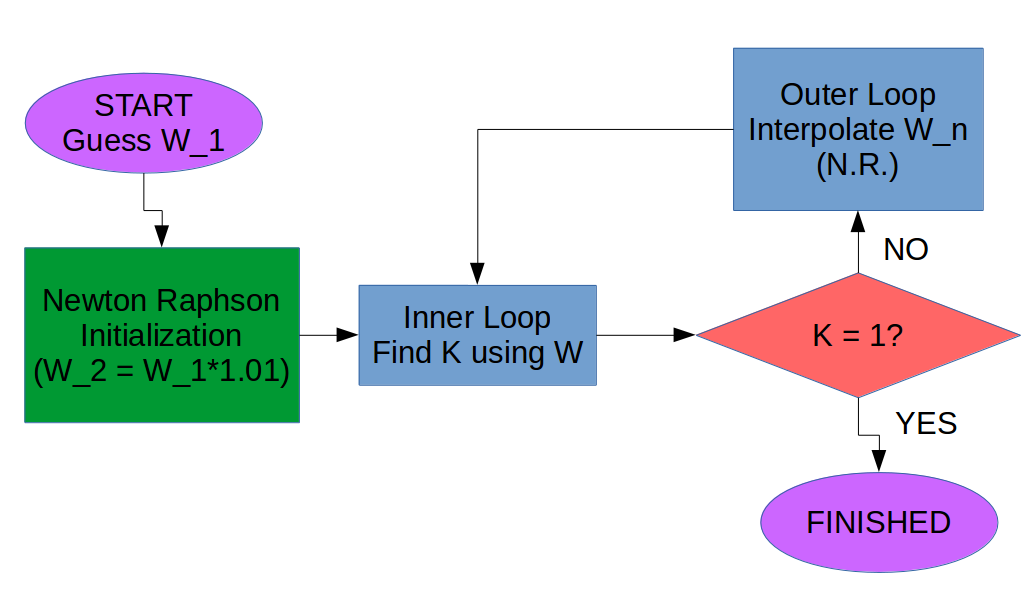
\includegraphics[width=\linewidth]{flow2.png}
				\label{flow}
			\end{figure}
		
	\section{Results}
		
		
	\section{Group Contributions}
		All project parts were worked on by all group members.		
\end{document}		